 \section{Plasticity and mechanical testing}
 
 \subsection{Dislocations}
  \FloatBarrier
In the IA course the behaviour of dislocations was covered in quite some detail, so this section will review and extend this.
 
To recap briefly, dislocations are linear defects that exist in crystalline materials and allow plastic deformation to occur. They are always of a slip system, which are defined by a slip direction, the relative displacement of atoms that result from their passage, and a slip plane, in which the dislocations move and across which the displacement happens, the displacement is the Burgers vector.
 
There are types of dislocations defined by the relative orientation of their line vector and Burgers vector, edge dislocations have their Burgers vector perpendicular to their line vector, while for screw dislocations these are parallel. For the purposes of this course we will mostly consider edge dislocations, though most of the analysis can be adapted to apply to screw dislocations.
 
In IA course E, the motion of dislocations was introduced as the mechanism that controls the strength of crystalline materials. The lower bound on strength was the lattice resistance or Peierls-Nabarro stress. Additionally, a number of strengthening mechanisms were introduced including:
\begin{itemize}
\item forest hardening
\item grain boundary hardening
\item solid solution strengthening
\item precipitate strengthening
order hardening
\end{itemize}

\begin{figure}[h!]
\centering
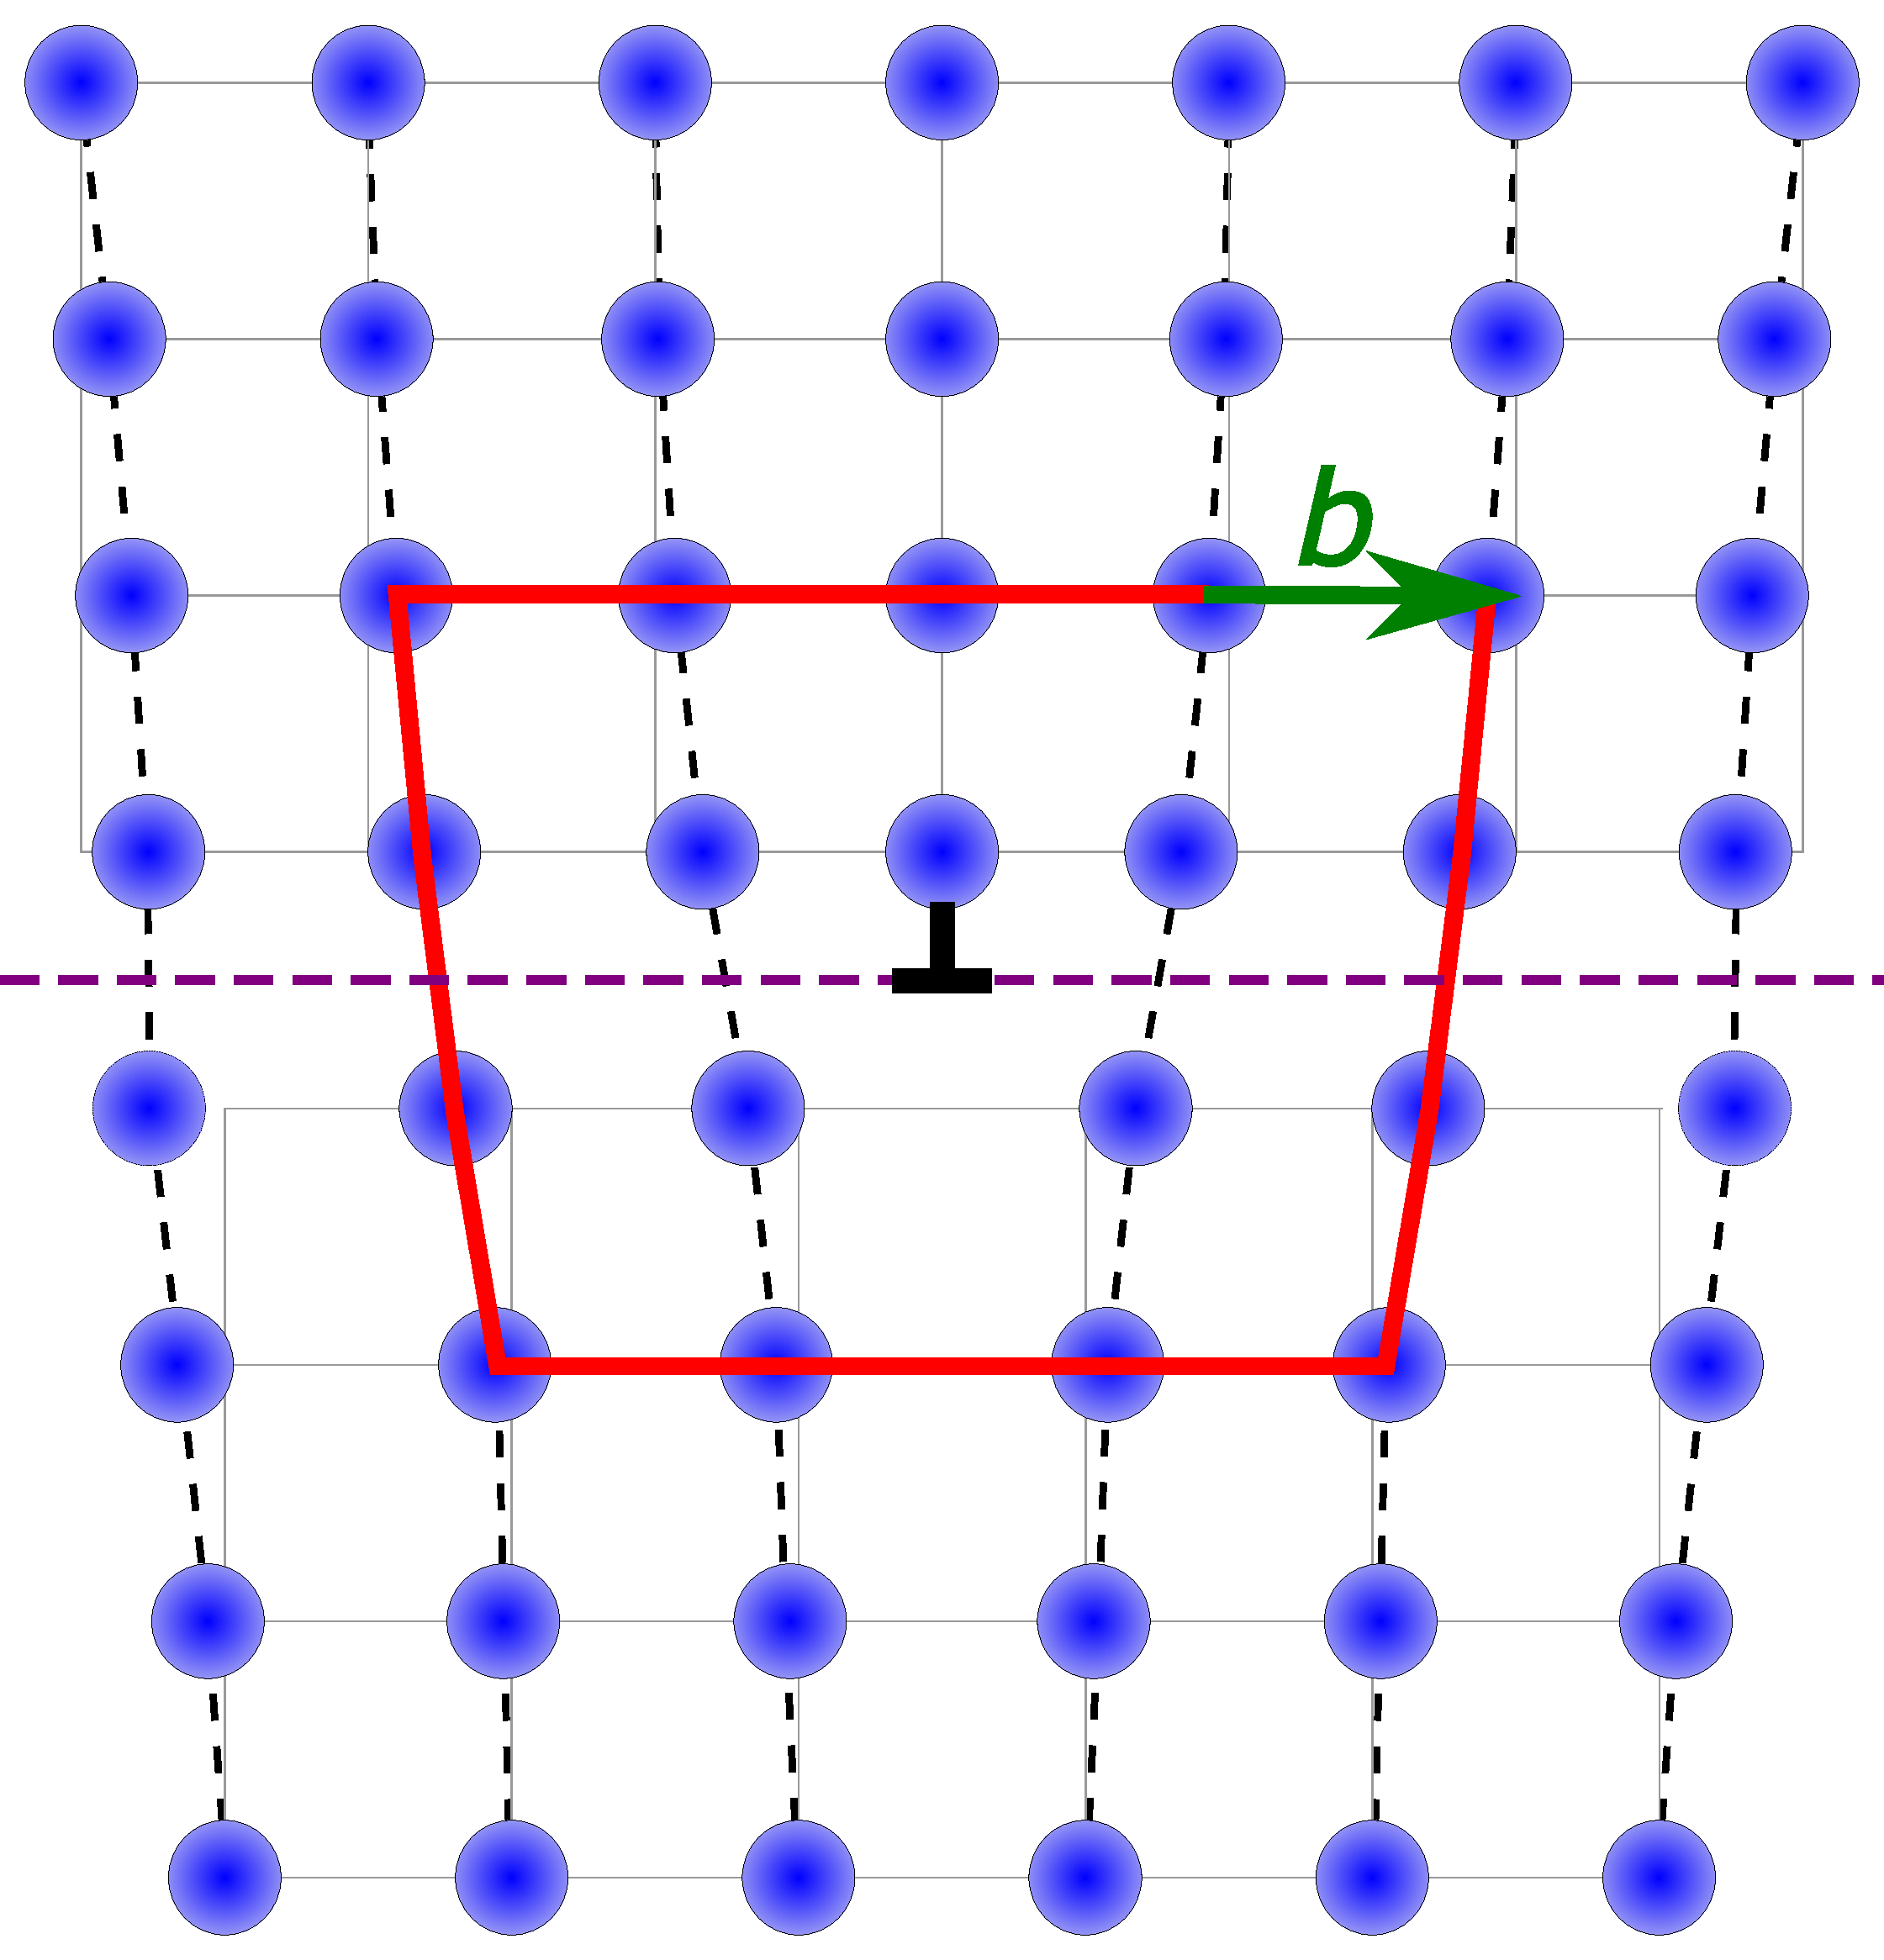
\includegraphics[width=0.6\textwidth]{Edge_Dislocation}
\caption{A schematic showing an edge dislocation, with the loop determined by a Burgers circuit. The slip plane is highlighted by the horizontal dashed line.}
\end{figure}
 
 
Here we will take a more in depth look at the lattice resistance and the way that work hardening occurs through the development of a dislocation network, introduced in IA as forest hardening.
\FloatBarrier

\subsubsection{The lattice resistance}

Dislocations were first considered as discontinuities in elastic continua, such a dislocation is called a ``Volterra'' dislocation. They are one of the classic problems of traditional continuum linear elasticity, however they cannot predict the behaviour of defects in a crystal which exist in a lattice.

It is precisely the periodicity of the crystal lattice that gives rise to a critical stress required to move a dislocation. The energy of a dislocation is not fixed, but will change as the dislocation moves with the same periodicity as the crystal lattice.

The energy changes associated with moving a dislocation were first examined mathematically by Rudolf Peierls and extended by Frank Nabarro. Their models have a common first step in examining the energy changes, which is to first calculate the energy of a dislocation.

\subsubsection*{Building a dislocation}
A dislocation can be created in a thought experiment by starting with two misaligned half crystals which are brought together at what becomes the slip plane.

The unit cells that span the slip plane will be experiencing large strains that will have a large associated energy. If we assume that the displacements normal to the slip plane are negligible, then there are two main components to the energy of either defects shown in \autoref{fig:making_a_disloc}: firstly there is a misalignment, essentially a shear strain across the slip plane with atoms displaced parallel to the slip with respect to the equilibrium neighbour across the slip plane. Secondly there will be a normal strain parallel to the slip plane, i.e.\ where the displacement parallel to the slip plane has brought neighbours {\bf in the same plane} too close together or too far apart.


\FloatBarrier
\begin{figure}[h!]
\centering
\begin{subfigure}{0.35\textwidth}
\centering
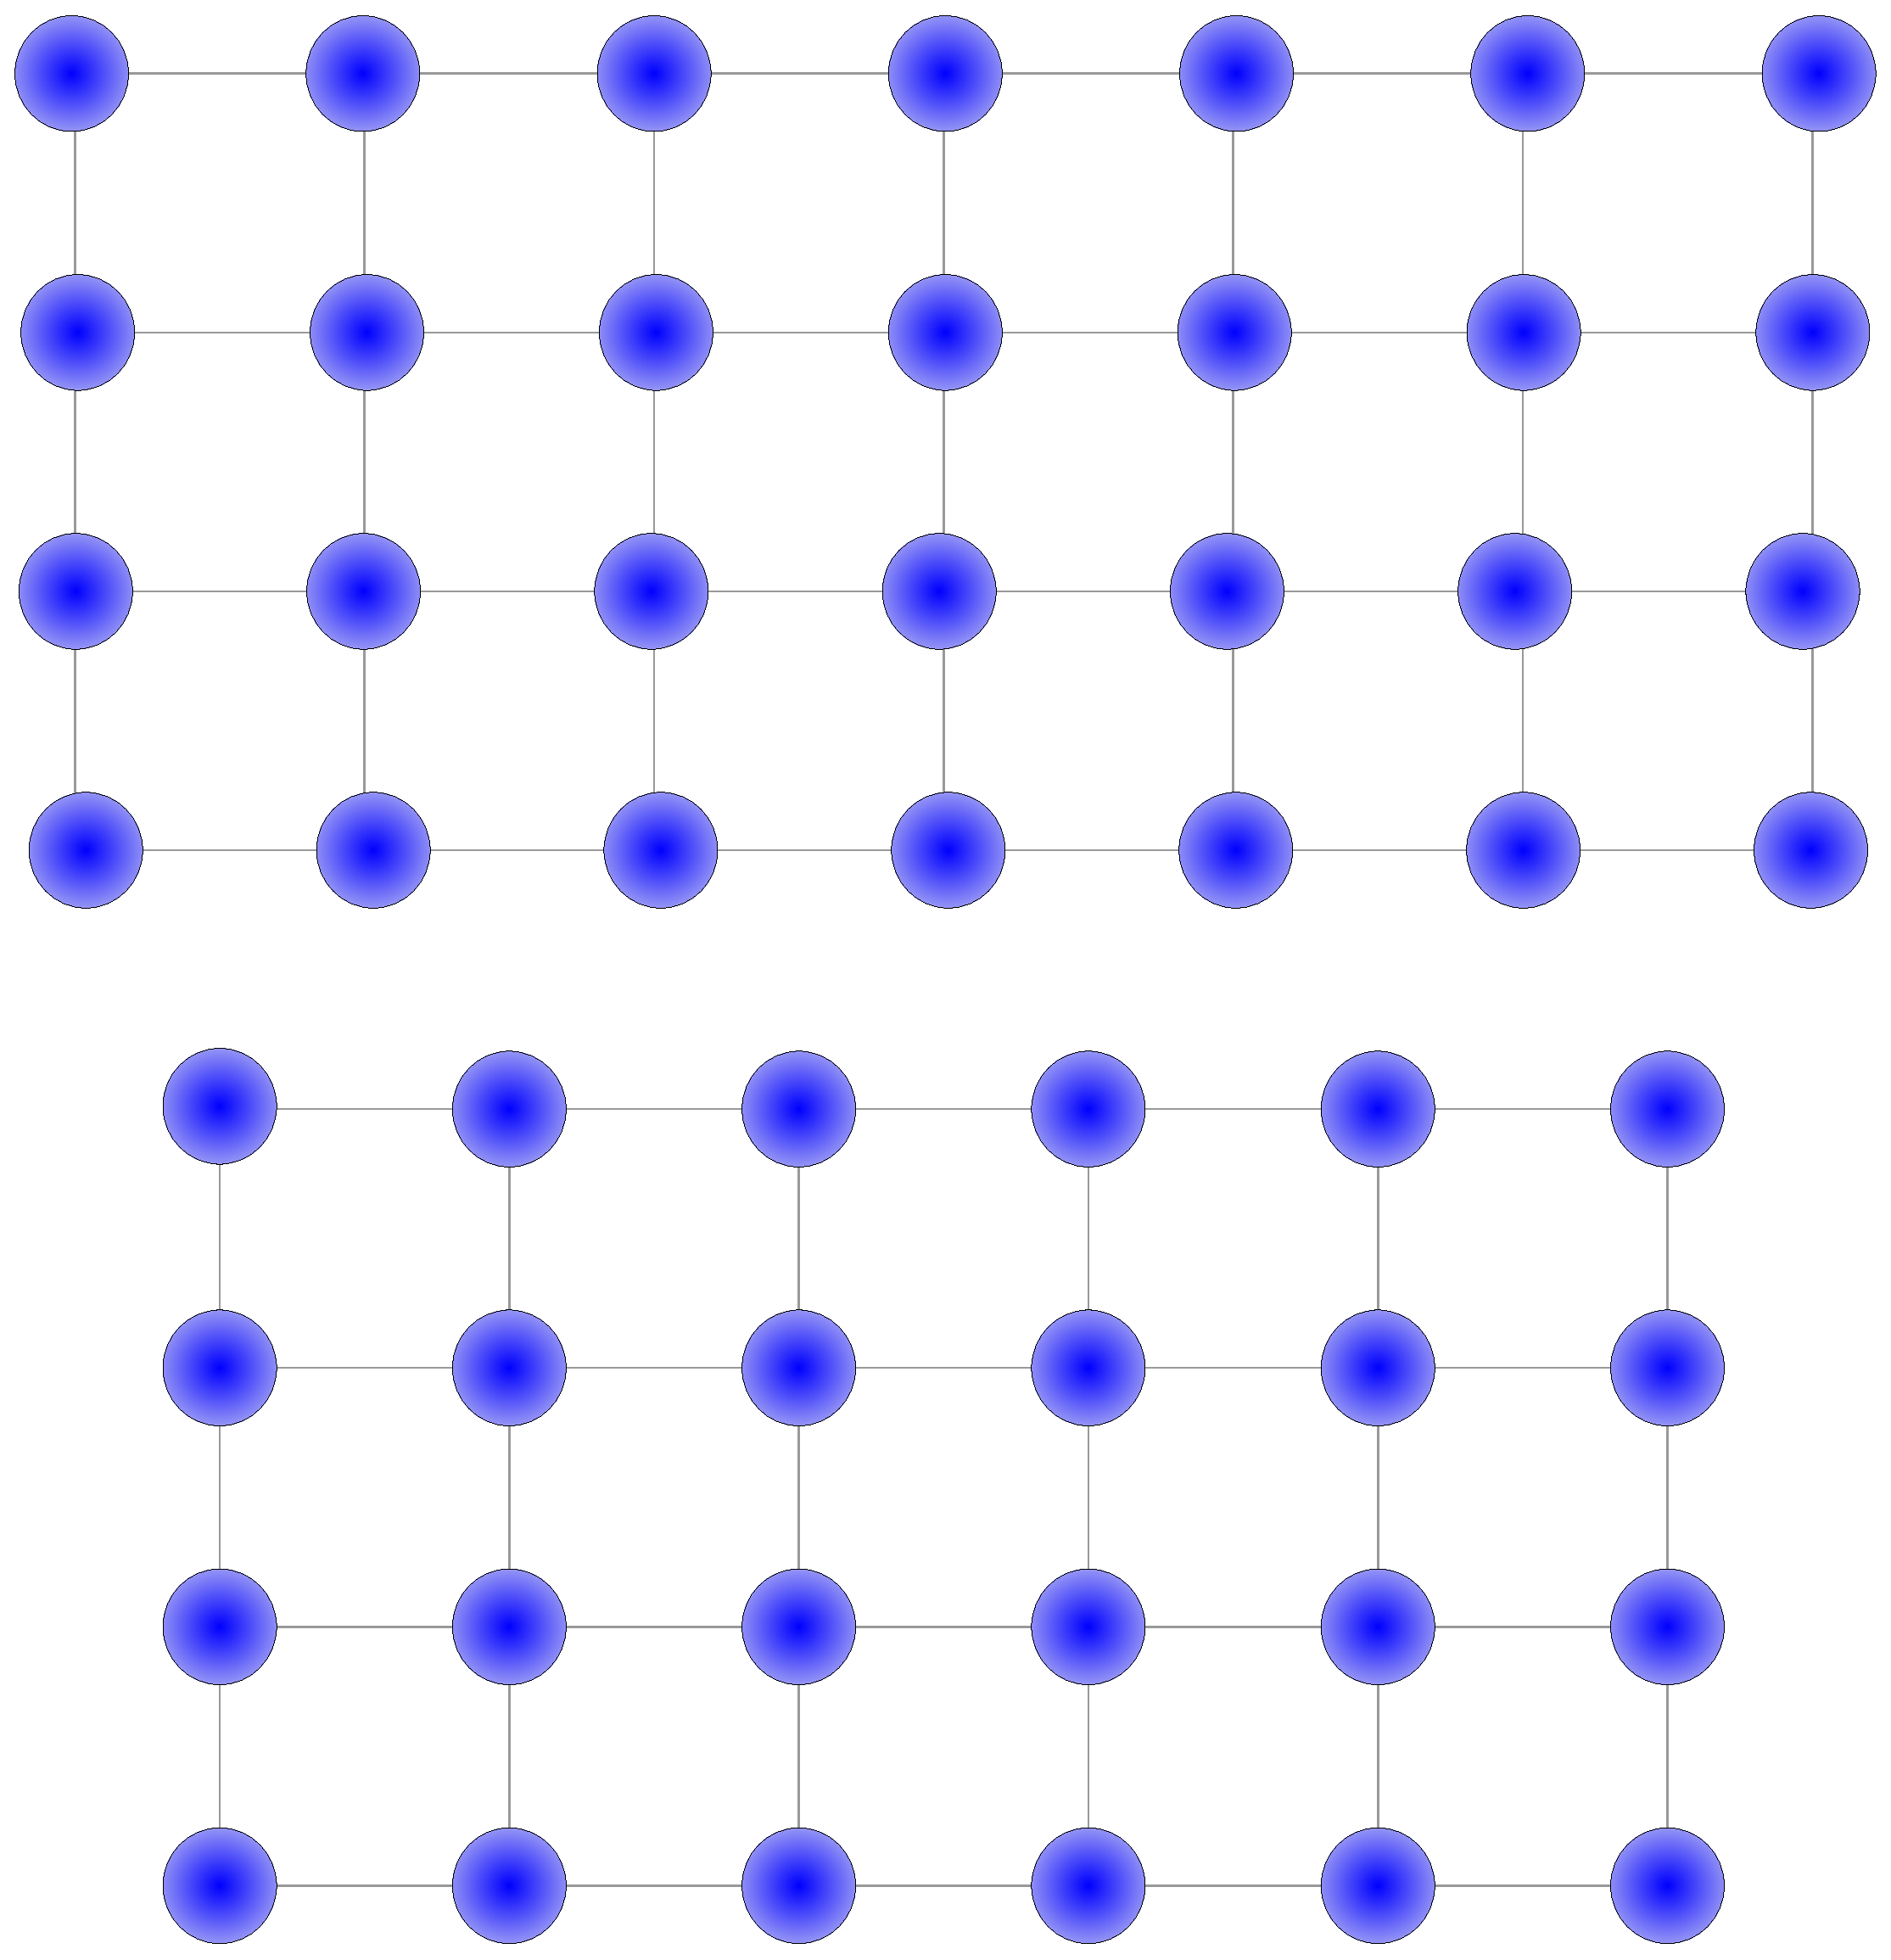
\includegraphics[width=\textwidth]{Half_crystals}
\caption{Two semi-infinite crystals misaligned by half of one Burgers vector. There is a planar defect between them.\label{fig:planar_defect}}
\end{subfigure}
~
\begin{subfigure}{0.35\textwidth}
\centering
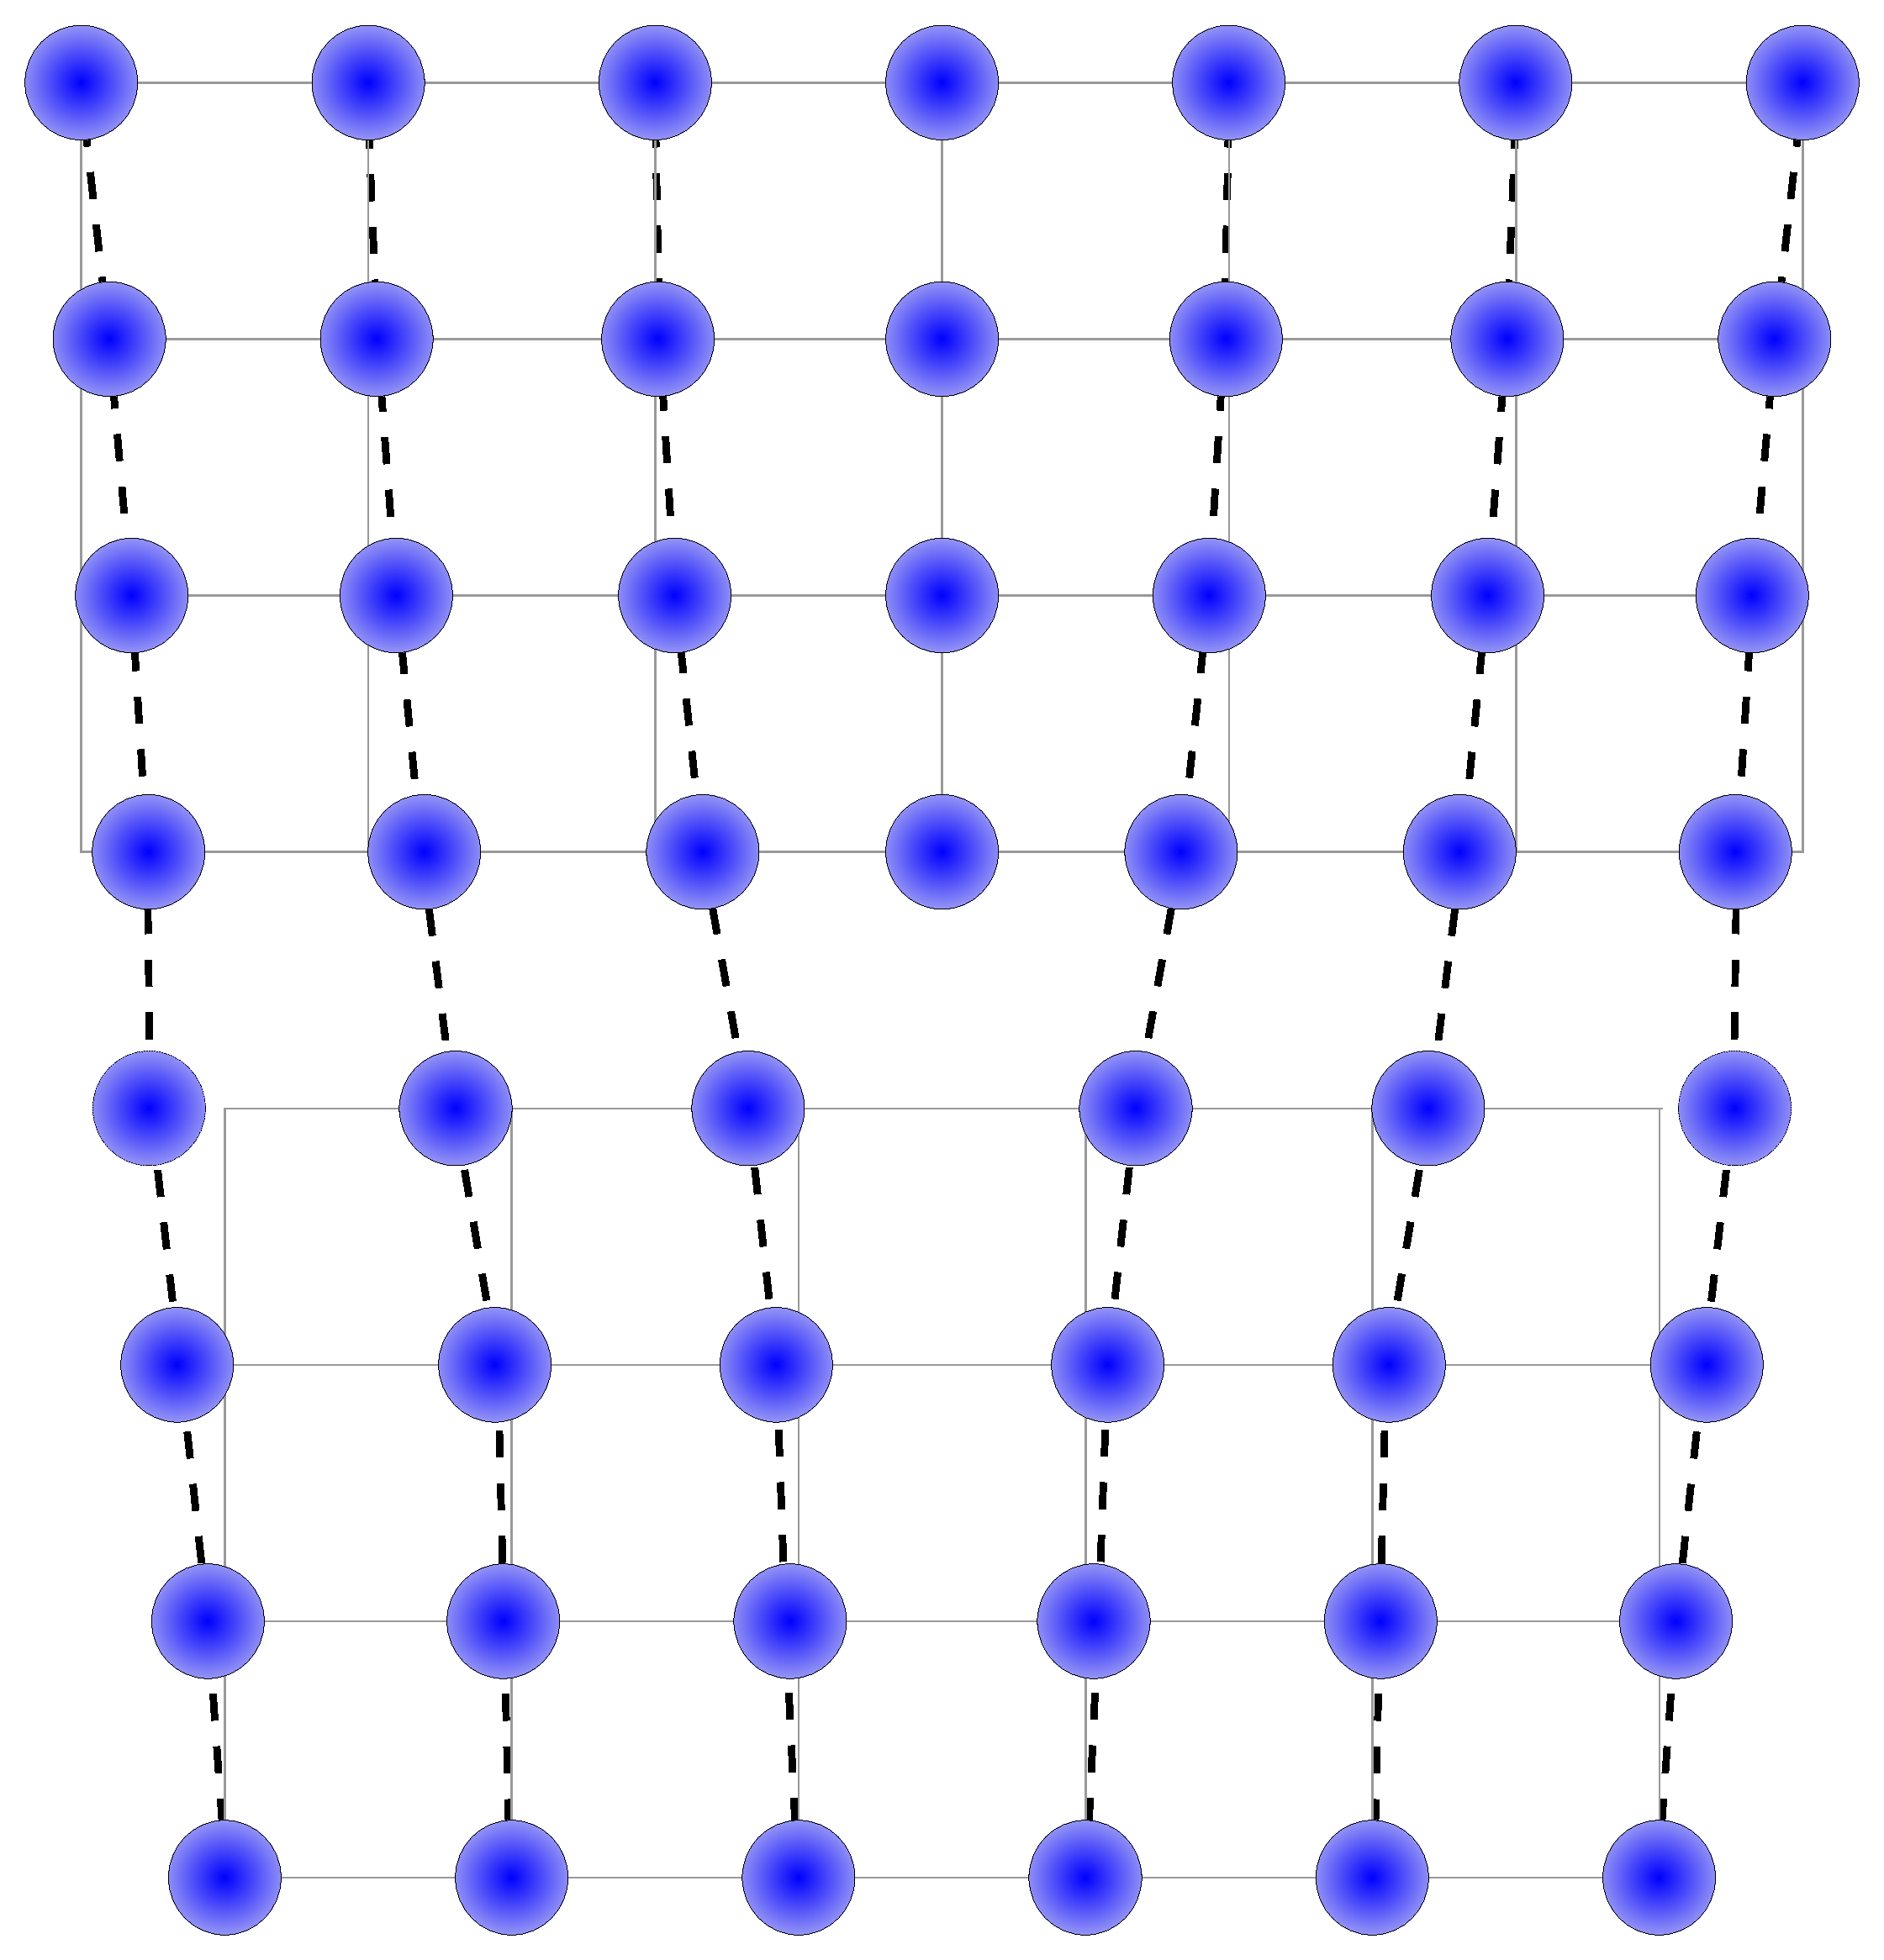
\includegraphics[width=\textwidth]{Edge_Dislocation_blank}
\caption{The atomic positions relax to form a dislocation, localising the strains and forming a linear defect.\label{fig:linear_defecct}}
\end{subfigure}
\caption{The formation of a dislocation, i.e.\ a line defect, from a planar defect.\label{fig:making_a_disloc}}
\end{figure}

\FloatBarrier
These two components favour different geometries of defect. In the case of the planar defect, the misalignment energy is at a maximum since the maximum number of cells are sheared the maximum amount, but the normal in-plane energy is at a minimum, in fact it's zero. In contrast localising the strains by aligning atoms across the slip plane will reduce the misalignment energy but increase the in-plane energy. The sum of these competing components will therefore pass through a minimum where the zone with large misalignments has a width that is neither zero or infinite. These two strain components, and the displacements that cause them are shown in \autoref{fig:peierls_details}.




\begin{figure}
\centering
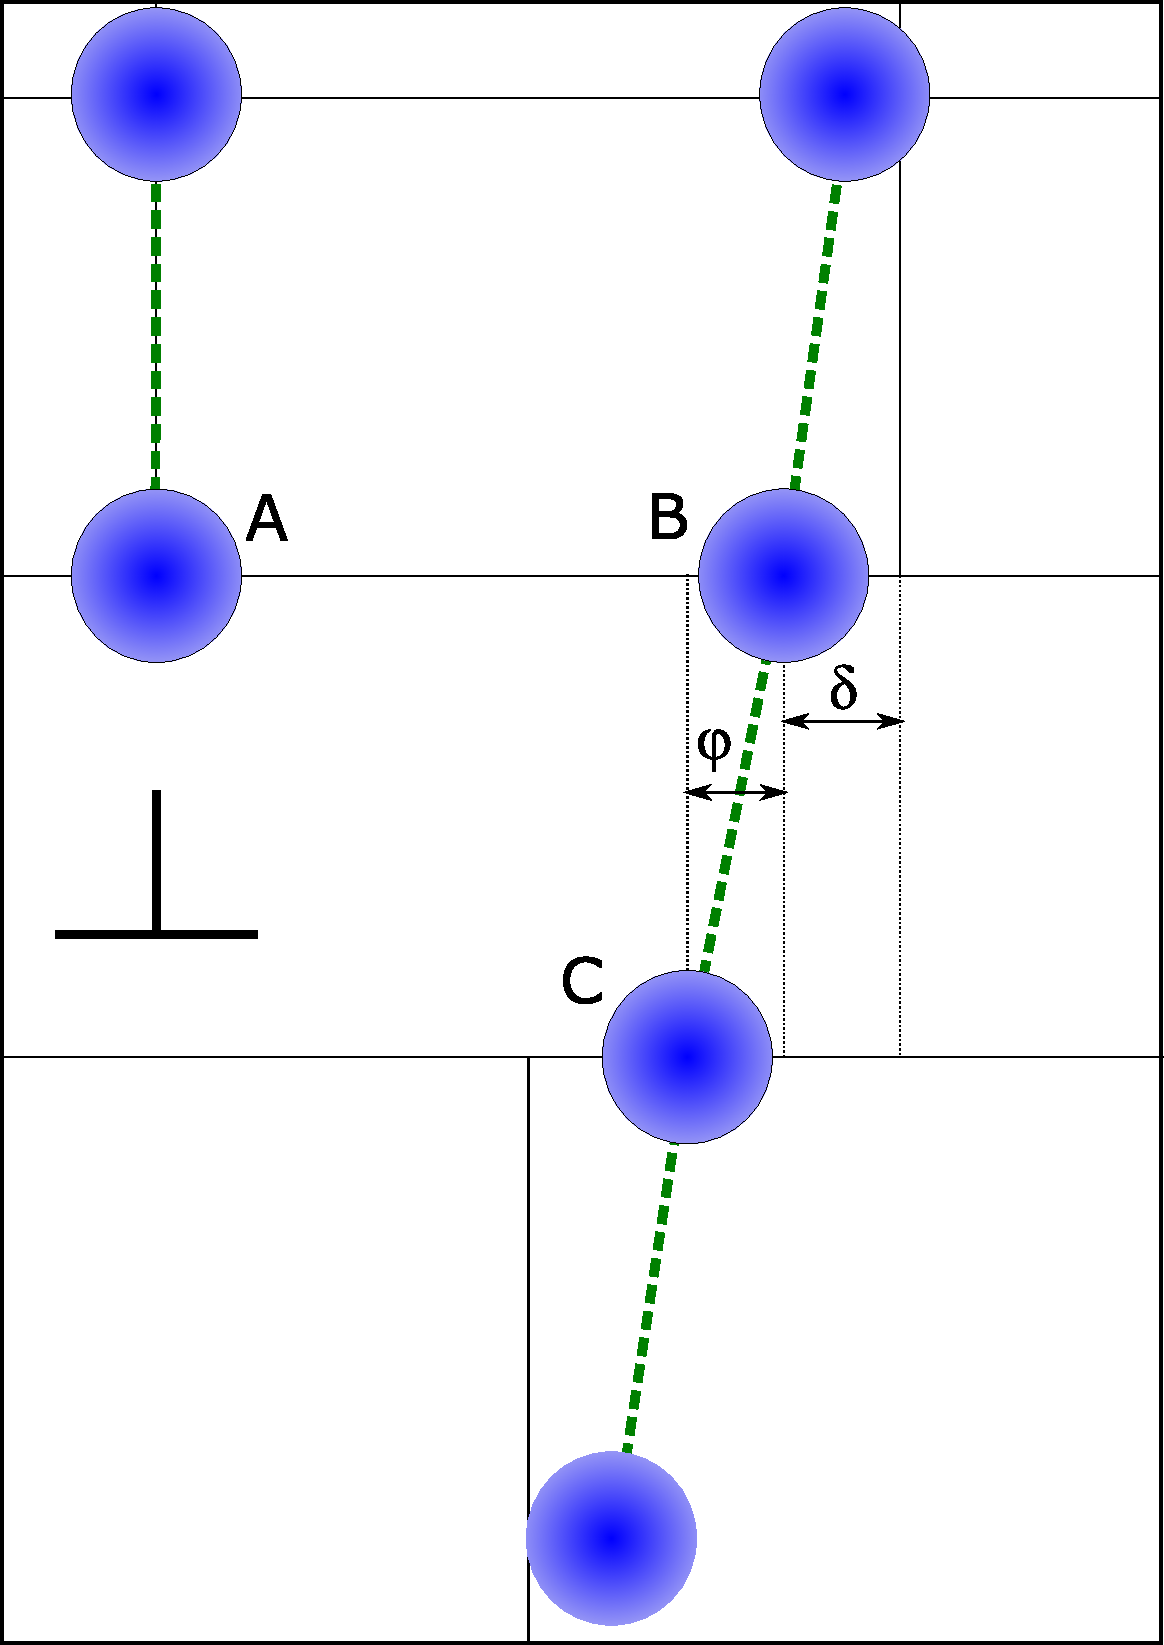
\includegraphics[width=0.5\textwidth]{peierls_model_detail}
\caption{The details of the relative displacements of atomic positions that give rise to strains around the core of a dislocation.\label{fig:peierls_details}}
\end{figure}

Using the displacements as defined in \autoref{fig:peierls_details}, and taking the equilibrium spacing to be $b$ parallel to the slip plane, and $d$ perpendicular to it, we can calculate the energy of the ``bonds''.

First the normal strains, caused by the displacement $\delta$, we can make the assumption that the energy is described by linear elasticity. Superficially this appears to imply that the energy should be $U_\text{i}=0.5E\varepsilon^2$. However this is not quite accurate, we need to account for the poisson strains, and any constraints on them.

\FloatBarrier
We start with the constitutive equations for an isotropic material (we'll make the assumption that the material is elastically isotropic for simplicity):

\begin{align*}
\varepsilon_1 = \frac{\sigma_1}{E} - \nu \frac{(\sigma_2 + \sigma_3)}{E} \\
\varepsilon_2 = \frac{\sigma_2}{E} - \nu \frac{(\sigma_1 + \sigma_3)}{E} \\
\varepsilon_3 = \frac{\sigma_3}{E} - \nu \frac{(\sigma_1 + \sigma_2)}{E} 
\end{align*}

I will define the 1, 2 and 3 directions relative to the edge dislocation such that the 1-axis is parallel to the Burgers vector, the 2-axis is parallel to the slip plane normal and the 3-axis is parallel to the line vector.


We can apply some boundary conditions to this situation. The symmetry of the dislocation line means there are now strains along the line, hence $\varepsilon_3 = 0$. We can also say that there is no physical reason to constrain the motion of atoms normal to the slip plane (at least as a first order approximation, neglecting the effect of strain gradients), so we can say that $\sigma_2 = 0$.

The former of these constraints gives us:
\begin{align*}
\frac{\sigma_3}{E} - \nu \frac{(\sigma_1 + \sigma_2)}{E} &= 0 \\
\sigma_3 - \nu \sigma_1 &= 0 \\
\sigma_3 &= \nu \sigma_1
\end{align*}

The positive sign here makes sense; the material would naturally contract (i.e.\ a negative strain) due to a perpendicular tension, but if constrained must be under a tension to oppose that effect.

Substituting back into $\varepsilon_1$:
\begin{align}
\varepsilon_1 &= \frac{\sigma_1}{E} - \nu \frac{(0 + \nu \sigma_1)}{E} \nonumber\\
&=\frac{\sigma_1 (1-\nu^2)}{E}\label{eqn:strain_one}
\end{align}

We can then use the equation for strain energy:
\begin{align*}
U &= \dfrac{1}{2} \varepsilon_i \sigma_i \qquad\begin{annotation}
\text{Note the summation convention over}\quad i=1,2,3 
\end{annotation}\\
U &= \dfrac{1}{2}(\varepsilon_1 \sigma_1 + \varepsilon_2 \sigma_2 + \varepsilon_3 \sigma_3)
\end{align*}

We know from the diagram in \autoref{fig:peierls_details} that $\varepsilon_1=\delta/b$ and since $\sigma_2=0$ and $\varepsilon_3=0$, we need only consider the first term. So rearranging \autoref{eqn:strain_one} and substituting for $\sigma_1$ we can write:
\begin{align}
U=\dfrac{1}{2} \varepsilon_1 \frac{E\varepsilon_1}{1-\nu^2} \nonumber\\
U= \frac{E}{2(1-\nu^2)}\varepsilon_1^2
\end{align}
This is in units of \si{\joule\per\meter^3}, if we want to consider the energy of a dislocation we must consider the energy per unit length, so we must multiply this volume energy by the area that lies perpendicular to the line length, i.e. $A= bd$, and substituting $\varepsilon_1 = \delta/b$:

\begin{equation}
U_{\text{line}} = \frac{E}{2(1-\nu^2)}\delta^2 \,\frac{d}{b}
\end{equation}

The energy of bonds misaligned across the slip plane are not so easily derived from first principles (albeit with some assumptions). Instead the best first approximation is not so much to make some assumptions as to take a large leap of faith. We assume that the small region of misaligned slip plane can be treated as a generalised planar fault. In IA the idea of stacking faults has been introduced, e.g.\ twinning in f.c.c. metals like Cu, or faults trailing a partial dislocation. 

These sorts of faults have generally have fixed offsets, for example in a ccp metal the usual stacking sequence is ...ABCABC... so a stacking fault might be ...ABCBA... where a plane that should be an A plane is a B plane, so there is a fixed misalignment equal to the displacement between those two sites. The concept can be generalised to a completely continuous misalignment from aligned through some sort of maximum misalignment and then returning to zero when the next site become aligned





\clearpage







\subsection{plasticity of isotropic materials}
The application of a tensile stress to an isotropic material produces perpendicular contraction stresses:
\begin{equation}
\varepsilon_{2} = \varepsilon_{3} = - \nu \varepsilon_{1}
\end{equation}
This gives the dilatation, or volume strain, as:
\begin{equation}
\Delta = \varepsilon_1 + \varepsilon_2 + \varepsilon_3 = \varepsilon_1 (1 - 2\nu)\label{eqn:volume_change_poisson}
\end{equation}
 
For most structural materials like metals, $\nu \approx 0.3$ and so for a strain of around \SI{0.5}{\percent} there is a volume change of around \SI{0.2}{\percent}. \autoref{eqn:volume_change_poisson} shows that as $\nu$ approaches 0.5 the volume change will approach zero.
 
However during plastic deformation there is no volume change